\scanpage{24}\mspage{18}
% @ top, check to make | text | À vérifier Les racines
\uline{À vérifier} Les racines $r_b$ orthogonales à un $u\in C$ (au nb de 40) forment un syst. de racines de type $D_5$

% @ upper third, NB | text | La donnée de (C,u,b)
\uline{NB} La donnée de $(C,u,b)$ avec $\unsure{u|b}\in C$, $b$ base ``orthogonale'' à $u$, équivaut à la donnée d'un ens $I$ de cardinal 6 (savoir $b$) et d'une partie \inserted{de $I$} $I_2$ de cardinal 2, i.e. \deleted{\unsure{de}} d'un ens \inserted{$I_2$} de cardinal 2 et d'un autre $I_4$ de cardinal 4. \deleted{Pour un système $(C,u,\{b,b'\})$, il faut se donner} \inserted{Groupe d'autom $\unsure{\mathfrak S|\mathscr S}_2\times\mathfrak S_4$,} nb $27\times40$ -- on a bien
% @ upper middle, order | display | Card W
\[
\operatorname{Card}W=(27\times40)\times(2.4!)=\unsure{27|2^7}.3^3.5
\]
% @ upper middle, opposite bases | text | Pour un syst.
Pour un syst. $(C,u,\{b,b'\})$, $\{b,b'\}$ bibase orth. à $u$, il correspond à $(I_2,I_4,\overset{\{b,b'\}}{J})$ $J$ un ens de Card. 2, Autom $\mathfrak S_{\underline{2}}\times\mathfrak S_4\times\mathfrak S_2$, il y en a $27.\frac{40}{2}$ \ldots.

% @ centre, separating flourish | drawing | broad horizontal zigzag with curved tail
\figure{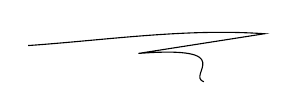
\begin{tikzpicture}[x=1cm,y=1cm]\draw (0,0)..controls(1,.07) and (2,.22)..(3,.15)--(1.4,-.10)..controls(2.7,.0) and (2,-.38)..(2.23,-.46);\end{tikzpicture}}

% @ lower half, heading | text | Graphes cubiques à arête marquée
\uline{\unsure{Graphe cubique|Graphes cubiques|Complexes cubiques} à arête marquée} (ou à triangle marqué avec sommet distingué)

% @ lower left, beside text | diagram | u, v, w ; heavy dot at u
\diagram{\begin{tikzcd}[ampersand replacement=\&,execute at end picture={
\draw (0,0)node[left]{$u$}--(1.03,.85)node[above]{$v$}--(1.27,.25)node[right]{$w$}--cycle;
\fill (0,0) circle (2.1pt);
}]\vphantom{A}\end{tikzcd}}

% @ lower half, construction | text | La description de cette structure
La description de cette structure se déduit de la description précédente en termes de $\{P_u,P\text{ torseur sous }\Psi_{Q_u}\}$ en se donnant de plus un élément fixé \inserted{$t$} de $Q_u$, de sorte que la donnée de $Q_u$ \inserted{de cardinal 5} revient à celle de $Q_u-\{t\}\deleted{\unsure{\mathrm{de}}}=P_u$ de cardinal 4. Alors
% @ lower third, projection below isomorphism | diagram | Ψ(Qᵤ), F₂ to powers Pᵤ and Qᵤ
\diagram{\begin{tikzcd}[ampersand replacement=\&,row sep=tiny]
\Psi(Q_u)\arrow[r,"\sim"]\arrow[r,phantom,"\deleted{\unsure{\simeq|\leftarrow}}"{above,pos=.22}] \&\mathbb F_2^{P_u}\\
\mathbb F_2^{Q_u}\arrow[u,phantom,"\subset"{description,rotate=-18}]\arrow[ur,"\mathrm{proj}"'] \&
\end{tikzcd}}
% @ lower third, torsor | text | donc la donnée du torseur
, donc la donnée du torseur $P$ sous $\Psi(Q_u)$ équiv. à celle d'un torseur $P$ sous $\mathbb F_2^{P_u}$ -- i.e. \inserted{$(P_u,P)\longleftarrow$} un ens. \inserted{$\widetilde P_u$} de cardinal 8 avec $\sigma$ autom involutif ss pt fixe.

% @ foot, augmentation | text | Considérons ε
\deleted{Alors} \deleted{\unsure{SPS}} Considérons $\varepsilon:\mathbb F_2^{P_u}\longrightarrow\mathbb F_2$, alors on a
% @ foot, decomposition | display | C as disjoint union
\[
C\simeq\{u\}\amalg\overbrace{\bigl(P\times_{\mathbb F_2^{P_u}}(\mathbb F_2,\varepsilon)\bigr)}^{\{v,w\}}
\amalg\deleted{\unsure{P}}\overbrace{\left(\coprod_{i\in P_u}\bigl(P\times_{\mathbb F_2^{P_u}}(\mathbb F_{2},p_i)\bigr)\right)}^{\widetilde P_u}
\amalg\overbrace{P}^{E}
\]
% archive sheet number: 23
